\documentclass[11pt,a4paper,titlepage]{article}
\usepackage{graphicx}
\usepackage[a4paper, total={6in,8in}]{geometry}
\DeclareGraphicsExtensions{.png}
\DeclareGraphicsExtensions{.jpg}

\begin{document}
\begin{titlepage}
	\begin{center}
		
		\begin{figure}[t]
			\centering
			
\includegraphics[width=350px, height=7cm]{images/thinkTechLogo.jpg}
		\end{figure}	
	
	\begin{flushright} 
		
		\textbf{\LARGE COS301 Main Project}
		\newline \newline \newline
		\textbf{\LARGE Flowchart Simulation Tool User Manual}
		\newline \newline \newline
 		\textbf{\LARGE ThinkTech}
		\newline \newline
	\end{flushright}
	
	\begin{flushright} \large
			
			\textbf{\LARGE Stakeholders}\newline 
			Lelethu Zazaza 13028023\newline
			Goodness Adegbenro 13046412\newline
			Hlavutelo Maluleke 12318109\newline
			Tshepiso Magagula 12274195\newline
			Xoliswa Ntshingila 13410378\newline
			
			
	\end{flushright}
	
	\begin{flushright} \large
	
			\textbf{\LARGE Client}\newline 
			Mr Willem S. van Heerden \newline
			University of Pretoria (Junior Lecturer)\newline
			
	\end{flushright}
		
		\vspace{1 cm}
		

		
		\vfill
		
		{\LARGE Version 0.2}
		\\
		{\large \today}		
		
		
	\end{center}
\end{titlepage}


\newpage
\tableofcontents
\pagenumbering{roman}
\newpage
\pagenumbering{arabic}
\section{System Overview}
	
		Flowchart Simulation Tool is an application which allows for designing and executing flowchart diagrams. A flowchart is a type of diagram that represents an algorithm, workflow or process, showing the steps as boxes of various kinds, and their order by connecting them with arrows (https://en.wikipedia.org/wiki/Flowchart). This diagrammatic representation illustrates a solution model to a given problem. Flowcharts are used in analysing, designing, documenting or managing a process or program in various fields. \newline
		
		This application is intended for academic purposes for first students with basic knowledge of programming design and implementation. This is a platform where the students can construct their own flowcharts, test and use them as they would like. \newline
		
		Furthermore, this system is highly related to the already existing edition of JavaBlock. The idea behind this system and that of JavaBlock is the same, they both pursue the same purpose. However, they are different when it comes to the usability of the system. With Flow (this system) focusing more on the interaction the user has on the system. For example, with JavaBlock to place a block onto the canvas one requires a couple of operations but with Flow, drag-and-drop operation is used.\newline
		
		Most importantly, this system is solely designed for the benefits of first-year students. However, it can also be extended for other relevant uses. For all other users, the purpose is still the same as other flowchart interpreters.
		
\section{System Configuration}
		
		This is desktop application, it is intended to operate on any Linux distribution. However, it can also be used on Windows platform. It is not a very sophisticated software and since the system is a minimal stand-alone application, not so many configurations required. \newline
		
		It is so far recommended that the computer in which the system will be executed on have Java 7 and above installed to allow the successful execution of the program. The system was not tested on Windows XP and the versions released before that, it is then recommended that the desktops should be running Windows 7 and above.\newline		
		
\section{System Installation}
		
		This system requires a complete installation in order to fully operate it. For different platforms, various installation files are required. \newline \newline
		
		The software can be found...
		
		% Create a website (or from sourceforge) 
		
		
		%---- link ----
		
		% Link and screenshots of the entire process until the user has the icon on the desktop
		

		\subsection{Windows installation}
		
		The image below shows the file that one requires for a complete successful installation of the program. Double-click the file to begin the installation process. \newline \newline \newline
		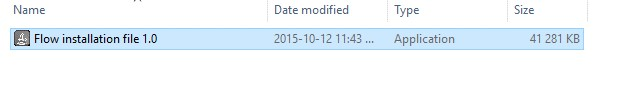
\includegraphics[width=13cm, height=2cm]{images/Install1.jpg}		
		\begin{center}
		Figure: The file used to install Flow \newline
		\end{center}
			
		Next, follow the installation prompts and complete the installation. After a successful installation the application will be added to computer programs and it is accessible from the start menu. \\ \\
		
		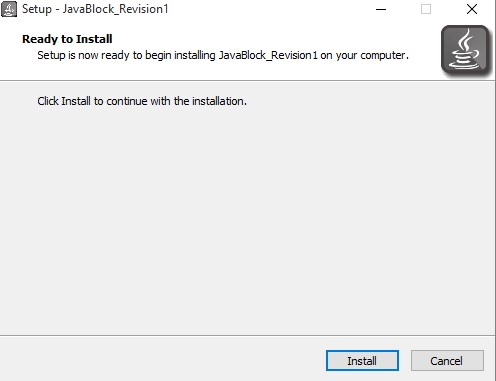
\includegraphics[width=13cm]{images/Install2.jpg}		
		\begin{center}
		Figure: Follow installation instructions
		\end{center}

\section{Getting Started}
	
	% For one to get to use the system, that particular user must be registered at the University of Pretoria, and have access to the Linux platform which is granted by the Department of Computer Science. From Linux, the user must be able to access the application, without any further installation or signing-up required.
	
	The sole purpose of this software was for first year students registered with the University of Pretoria to use as a flowchart simulator tool. However, it is also available for everyone else who wishes to use it for various purposes. Instruction on how to access the necessary files to install the software are provided above.\\
	\\For University of Pretoria students, the system will be installed in the Informatorium labs, they will be able to use it from the computers available in the Informatorium. Access to the computers in the Informatorium is restricted to specific students, these students are ones to have access to the system.\\

% This section forms the bulk of the user manual.


	
	\subsection{Running Software}
	
	% Screenshots of how the file should be exucuted	
	
		% The application will not require any installation. To run the application the user will only require the executable file which will be provided via the on-line University of Pretoria (Computer Science) website. With the executable file the user will only need to double click on the file, then the system will star-up.
		
	%	For the time being an executable .jar file has been created to allow instant execution of the system without any installation. Below its a simple outline which illustrate this, an executable is clicked on the top right of the screen and Flow appears instantly. \newline \newline
	
	
		After a successful installation of Flow, the potential user can then start the application normally on their machine. The image below depicts the desktop short-cut icon created after the installation is complete.	\\
		
		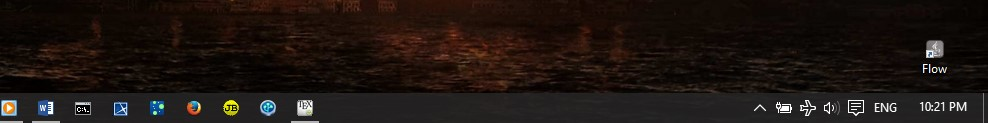
\includegraphics[width=14cm]{images/DesktopIcon.jpg}
		\begin{center}
			Figure: Flow desktop icon.\\
		\end{center} 
		
		
		Double-clicking the icon on the desktop will consequently open the application. More about the application is discussed below.
		
		
		\subsection{Software Layout}
		The layout is composed of the canvas, flowchart tools and menu options. The figure below depicts the general layout of the entire system.
		
		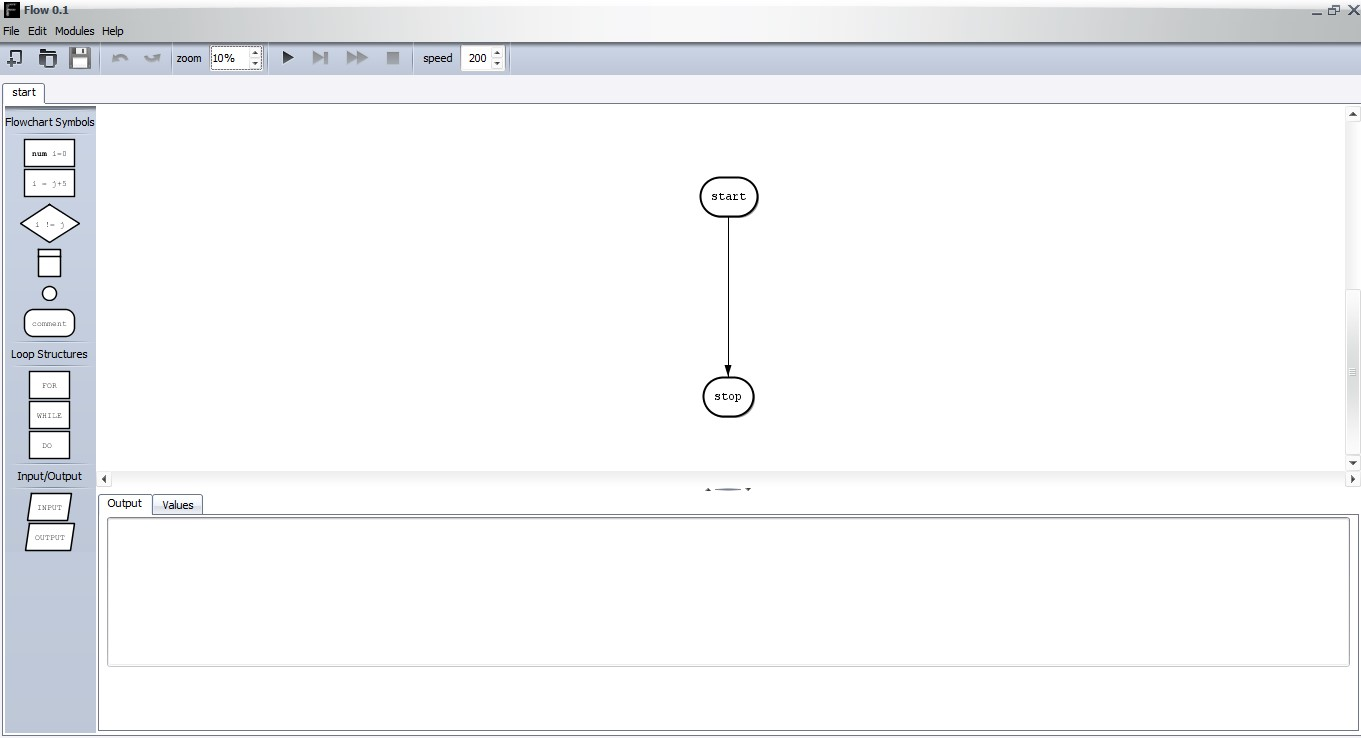
\includegraphics[width=\textwidth]{images/SystemLayout.jpg}
		\begin{center}
		Figure: The General System Layout.\newline
		\end{center}
		
		
		\begin{itemize}
			\item \textbf{Canvas:} This space is provided to design a 			well-formed flowchart. Components will be dragged from the flowchart 				tools menu consisting of available components and dropped onto the 				canvas. See figure below.\newline
			There are components which are already implemented at start of the system, the 'start' and 'end' blocks are initialised by default on the canvas.\newline \newline
			
\includegraphics[width=11.5cm]{images/Canvas.jpg}
			\begin{center}
		Figure: The Canvas.\newline
		\end{center}
			
			\item \textbf{Flowchart Tools:} This contains all the tools required to construct the flowchart. All the components will be dragged and dropped onto the canvas (as illustrated by the the figure below), with the tools on the left and the canvas on the right. All the necessary components to build a flowchart are listed on the left toolbar.\newline
			
		The tools are draggable, i.e, from the toolbar hover over the block you want to use and drag it over to the canvas (the white plane on the left - as illustrated above). Under "using the system" is a detailed illustration on how to use these tools. \newline \newline			
			
			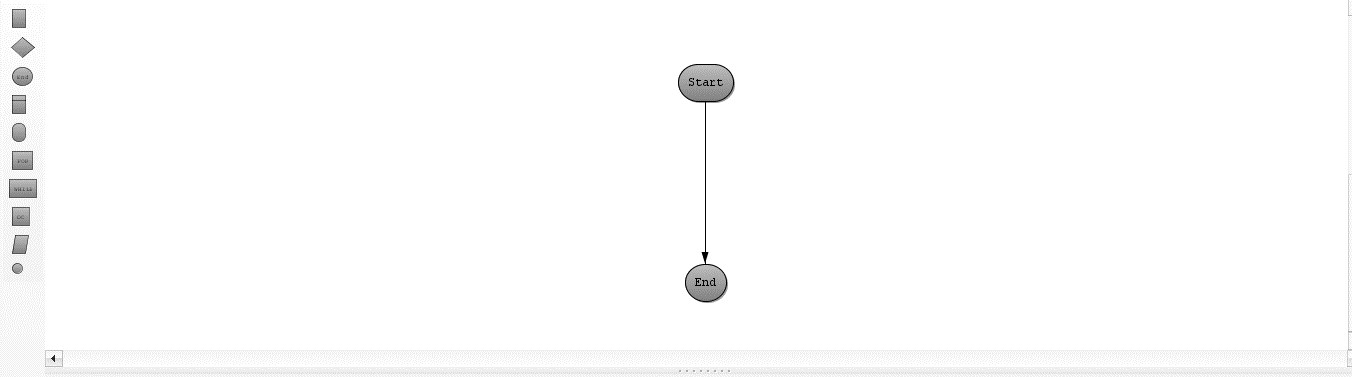
\includegraphics[width=11.5cm]{images/Tools.jpg}
			\begin{center}
		Figure: Flowchart Tool Components.\newline
		\end{center} 
			
						
			\item \textbf{Menu Options -} The menu option provides options of creating, saving, deleting and loading projects onto the canvas. Also, this provides the user with many more options which are accessible by hovering over the name of the option. The figure below shows the functionality of all this.\newline 
		
		\begin{itemize}
		\item Creating projects: The detailed description of this is given under "Creating projects"  below.
		\item Saving projects:  The detailed description of this is given under "Saving projects" below.
		\item Deleting projects: This will delete the entire project, from the main flowchart to the modules that the flowchart uses.
		\item Loading projects: The detailed description of this is given under "Opening existing projects" below.
\end{itemize}				
			
			
			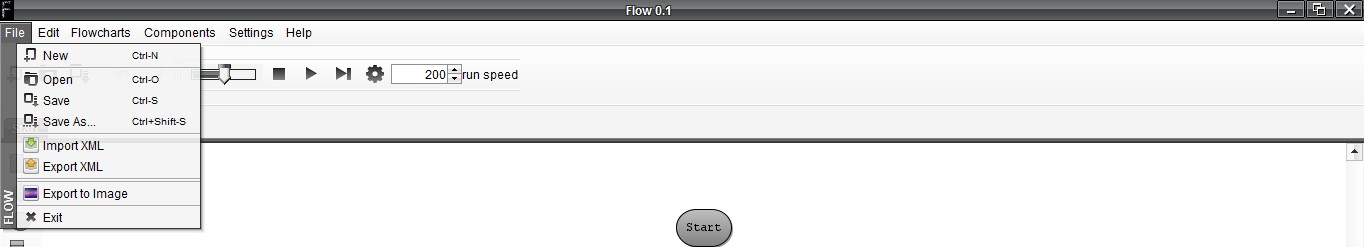
\includegraphics[width=11.5cm]{images/Menu.jpg}
			\begin{center}
		Figure: Menu Bar.
		\end{center}
			
			
		\end{itemize}

	\newpage
	
	
	
%%%%%%%%%%%%%%%%%% Very important %%%%%%%%%%%%%%%%%%%%%%%%%%%%%%%%%%%%%%
	
	
	
\section{Using the System}
	\subsection{Creating New Project}
	
	When the application is opened for the first time, a default project is created with a default flowchart, which compiles and execute without any output generated. The user then will start his/her own building of the flowchart from already generated default flowchart. This is also demonstrated by the figure on general flowchart layout. \newline\newline
However, the user can create new project from the menu bar. To create a new project select "File" in the menu bar and a drop down menu will appear. Select the "New" option, a pop-up window will appear requesting the desired file name for the project. Enter the file name and press the enter key on the keyboard, then the new project with the default flowchart will be created. \newline
		
		
	\subsection{Adding Components to Canvas}
	
	From the created project, construction starts with dragging the components from the tool bar to the canvas. Adding components to the canvas is quite simple, drag the desired component from the tool bar and drop it onto the canvas. The component will be locally saved on the canvas, continue doing so until the building is complete.
	
	\subsection{Editing Component}
	
	Editing the component entails manipulation of the features and adding code inside the component. To edit the component click on the component that you want to edit and the a pop-up window will appear on the far left side of the application with the options of changing features or adding code.
		
	\subsection{Removing Components from Canvas}
	
	To remove any component from the canvas right-click on the component and select delete component. To remove multiple components hold the "SHIFT" key and select the components and then right-click and select delete component.
		
	\subsection{Saving Project}
	
	To save your current progress go to "File" in the menu bar, in the drop down menu select "Save". Enter the name of the file and then the project will be saved in a directory for flowchart projects.
	
	\subsection{Run Simulation}
	To run the flowchart select the "Run" icon on the flowchart tools window and the the whole flowchart will execute. To run the flowchart step-by-step select the "Step" icon.
	
		
	\subsection{Opening Existing Project}
	
	To open an existing project go to the menu bar and select the "File" option and then select the "Open" menu item. Search for an existing flowchart project with the valid extention. The flowchart project will now be loaded onto the canvas and should be able to be updated.
	
\section{Troubleshooting}

Recall from "System Configuration" the Java version compatible with this system. Older versions of Java may cause the system to break, and not execute as expected. Hence, violating the reliability of the entire system.

This system is not connected to any other external systems, this reduces the amount of errors that might usually breakdown the system.

\end{document}